\documentclass[border=6pt]{standalone}
\usepackage{tikz}
\usetikzlibrary{decorations.pathreplacing}
\begin{document}
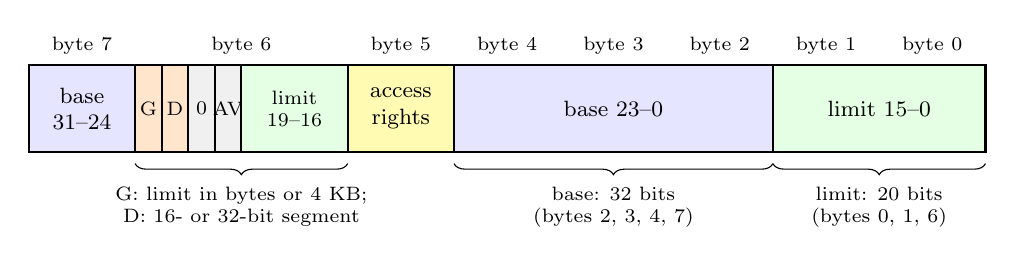
\begin{tikzpicture}[font=\small,x=1.35cm]
\foreach \b/\x in {7/0.5,6/2,5/3.5,4/4.5,3/5.5,2/6.5,1/7.5,0/8.5} \node[font=\scriptsize] at (\x,0.75) {byte \b};
\foreach \xa/\xb/\t/\c in {0/1/{base\\31--24}/blue!10,3/4/{access\\rights}/yellow!30,4/7/{base 23--0}/blue!10,7/9/{limit 15--0}/green!10} {
  \draw[thick,fill=\c] (\xa,-0.6) rectangle (\xb,0.5);
  \node[font=\footnotesize,align=center] at ({(\xa+\xb)/2},-0.05) {\t};
}
% byte 6 split into G, D, 0, AV, limit 19-16
\foreach \xa/\xb/\t/\c in {1/1.25/G/orange!20,1.25/1.5/D/orange!20,1.5/1.75/0/gray!12,1.75/2/AV/gray!12,2/3/{limit\\19--16}/green!10} {
  \draw[thick,fill=\c] (\xa,-0.6) rectangle (\xb,0.5);
  \node[font=\scriptsize,align=center] at ({(\xa+\xb)/2},-0.05) {\t};
}
\draw[decorate,decoration={brace,mirror,amplitude=4pt}] (1,-0.75) -- (3,-0.75) node[midway,below=5pt,font=\scriptsize,align=center]{G: limit in bytes or 4 KB;\\D: 16- or 32-bit segment};
\draw[decorate,decoration={brace,mirror,amplitude=4pt}] (4,-0.75) -- (7,-0.75) node[midway,below=5pt,font=\scriptsize,align=center]{base: 32 bits\\(bytes 2, 3, 4, 7)};
\draw[decorate,decoration={brace,mirror,amplitude=4pt}] (7,-0.75) -- (9,-0.75) node[midway,below=5pt,font=\scriptsize,align=center]{limit: 20 bits\\(bytes 0, 1, 6)};
\end{tikzpicture}
\end{document}
